\chapter{Un método HDG aplicado a la ecuación de Helmholtz.}
\section{Preliminares y dominio computacional.}
%%definiciones de conjuntos
\setstretch{1.5}
Para realizar el estudio del método HDG aplicado a la formulación \red{(AQUI FALTA)}, es necesario definir la notación a utilizar.
Primero se define
\[ \inner{\cdot}{\cdot}_{\TT_h} := \sum_{K \in \TT_h}{\inner{\cdot}{\cdot}_{K}} \quad,\quad \pdual{\cdot}{\cdot}_{\partial \TT_h} := \sum_{K \in \TT_h}{\pdual{\cdot}{\cdot}_{\partial K}} \quad,\quad  \pdual{\cdot}{\cdot}_{\partial \TT_h \backslash \Gamma} := \sum_{e \in \EE_h}{\pdual{\cdot}{\cdot}_{e}} .\]
Donde $\inner{\cdot}{\cdot}_K$, $\pdual{\cdot}{\cdot}_{\partial K}$ y $\pdual{\cdot}{\cdot}_{e}$ es el producto interior estandar de $L2$ sobre el elemento $K$, su frontera $\partial K$ y lado $e$, respectivamente. Sea $\lla{\mathcal{T}_h}_{h>0}$ una familia de triangulaciones {\sc shape-regular} de $\Omega$, formada por triángulos $K$ cuyos lados se denominan $e$, donde el diametro se denota por $h_K$ y $\bn$ es el vector normal exterior. También, sean $\dTT_h := \lla{\partial K : K \in \TT_h}$ y $\EE_h := \EE_o \cup \EE_t \cup \EE_b \cup \EE_l \cup \EE_r$, donde $\EE_o$, $\EE_t$, $\EE_b$, $\EE_l$, $\EE_r$ denotan los lados interiores, de frontera superior, inferior, izquierda y derecha, respectivamente.

Como el dominio es quasi-periódico, la partición $\EE_l$ induce una nueva partición sobre sobre la frontera derecha $\Gamma_r$, que denotamos por $\FF_r$. Del mismo modo, $\EE_r$ induce una nueva partición sobresla frontera izquierda $\Gamma_l$ que denotamos $\FF_l$. 

En otras palabras, sean $\NN_l := \lla{\pa{0,y_0}, \ldots , \pa{0,y_{N_l}}}$ el conjunto de nodos de la partición $\EE_l$ con $y_0 < y_1 < \ldots < y_{N_l}$ y $\NN_r := \lla{\pa{L,z_0}, \ldots , \pa{L,z_{N_r}}}$ el conjunto de nodos de la partición $\EE_r$ con $z_0 < z_1 < \ldots < z_{N_r}$. Una manera de poder hacer coincidir la cantidad de nodos en ambas nuevas particiones inducidas es considerar el conjunto $\lla{w_j}_{j=0}^N$ formado por la unión de $\lla{y_j}_{j=0}^{N_l}$ y $\lla{z_j}_{j=0}^{N_r}$ excluyendo repeticiones tal que $w_0 < w_1 < \ldots < w_{N}$. Así, las particiones inducidas se definen de la forma $\FF_l := \lla{\pa{0,w_0}, \ldots , \pa{0,w_{N}}}$ y $\FF_r := \lla{\pa{L,w_0}, \ldots , \pa{L,w_{N}}}$ de las fronteras $\Gamma_l$ y $\Gamma_r$ respectivamente.

\begin{figure}[H]
    \centering
    \begin{subfigure}[b]{0.45\textwidth}
        \centering
        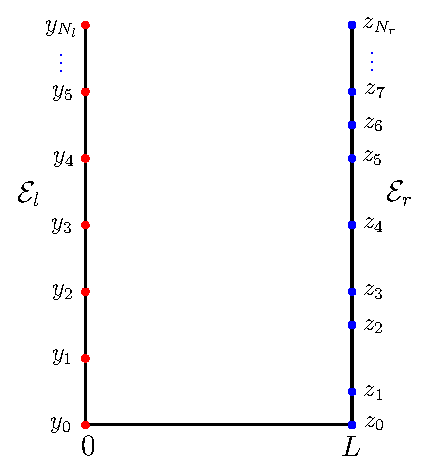
\includegraphics[scale=0.8]{./img/dom_1.eps}
        \caption{En rojo los nodos de $\EE_l$ y en azul los nodos de $\EE_r$.}
        \label{fig:domain_1}
    \end{subfigure}
    \hfill
    \begin{subfigure}[b]{0.45\textwidth}
        \centering
        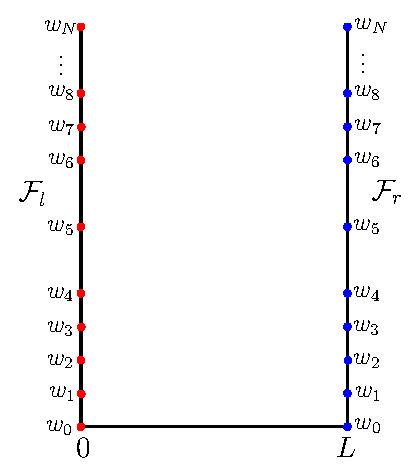
\includegraphics[scale=0.8]{./img/dom_2.eps}
        \caption{En rojo los nodos de $\FF_l$ y en azul los nodos de $\FF_r$.}
        \label{fig:domain_2}
    \end{subfigure}
    \label{fig:domain}
    \caption{Representación de las particiones.}
\end{figure}

Dado un elemento $K \in \TT_h$, un lado $e \in \EE_h$ y un entero no negativo $k$, $\P_k \pa{K}$ y $\P_k \pa{e}$ denotan los espacios de polinomios de grado menor o igual a $k$ sobre $K$ y $e$ respectivamente. También se define $\BP_k := \cor{\P_k \pa{K}}^d$. Luego, para $\ast \in \lla{l,r}$, denotamos $P_{\FF_{\ast}}^{k_\FF}$ a la proyección ortogonal $L^2 \pa{\Gamma_\ast}$ sobre $\P_{k_\FF} \pa{\FF_\ast}$.

\section{El esquema HDG.}
Introducimos los siguientes espacios discretos asociados a la triangulación $\TT_h$
\begin{align*}
    \BV_h &:=\lla{\bv \in \BL^2 \pa{\TT_h}: \left.\bv \right|_K \in \BP_k \pa{K} \quad \forall K \in \TT_h}, \\ 
    W_h &:= \pa{w \in L^2 \pa{\TT_h}:  \left. w \right|_K \in \P_k \pa{K} \quad \forall K \in \TT_h}, \\
    M_h &:= \lla{\mu \in L^2 \pa{\EE_h}:  \left. \mu \right|_e \in \P_k \pa{e} \quad  \forall e \in \EE_h}, \\
    M_h^{qp} &:= \lla{\mu \in M_h: P_{\FF_l}^{k_\FF} \pa{ \left. \mu \right|_{\EE_l}} = e^{i \alpha L} P_{\FF_r}^{k_\FF} \pa{ \left. \mu \right|_{\EE_r}} }. 
\end{align*}
